\documentclass{article}
\usepackage[utf8]{inputenc}
\usepackage[IL2]{fontenc}
\usepackage[czech]{babel}
\usepackage{titling}
\usepackage{indentfirst}
\usepackage{graphicx}
\usepackage{wrapfig}
\usepackage{subcaption}
\usepackage{caption}
\usepackage[style=alphabetic]{biblatex}
\usepackage{listings}
\usepackage{xcolor}
\definecolor{codegreen}{rgb}{0,0.6,0}
\definecolor{codegray}{rgb}{0.5,0.5,0.5}
\definecolor{codepurple}{rgb}{0.58,0,0.82}
\definecolor{backcolour}{rgb}{0.95,0.95,0.92}

\lstdefinestyle{mystyle}{
    backgroundcolor=\color{backcolour},   
    commentstyle=\color{codegreen},
    keywordstyle=\color{magenta},
    numberstyle=\tiny\color{codegray},
    stringstyle=\color{codepurple},
    basicstyle=\ttfamily\footnotesize,
    breakatwhitespace=false,         
    breaklines=true,                 
    captionpos=b,                    
    keepspaces=true,                 
    numbers=left,                    
    numbersep=5pt,                  
    showspaces=false,                
    showstringspaces=false,
    showtabs=false,                  
    tabsize=2
}
\lstset{style=mystyle}

\usepackage{amsmath}
\usepackage{amssymb}
\usepackage{amsthm}
\theoremstyle{definition}
\newtheorem{definition}{Definice}[section]

\usepackage{hyperref}
\hypersetup{
    colorlinks=false, %set true if you want colored links
    linktoc=all,     %set to all if you want both sections and subsections linked
}

\addbibresource{lit.bib}

\title{%
Semestrální práce - Benchmarkování knihovny pro kryptografii eliptických křivek \\
\large KIV/VSS
}
\author{Jakub Mladý \\ scrub@students.zcu.cz}

\date{Červenec 2023}

\begin{document}
\begin{titlingpage}
\begin{figure}
    
\includegraphics[scale=0.5]{fav_logo}
\end{figure}

\maketitle
\end{titlingpage}
\tableofcontents
\newpage

\section{Úvod}
Kryptografie je v dnešním digitálním světě užitečným nástrojem sloužícím mnoha různým účelům. Zajišťuje soukromí posílání zpráv pomocí šifrování, bezpečnou výměnu klíčů pro šifry, ověřování integrity dat hešováním a autentizaci protistrany při komunikaci. Chrání anonymitu a přesto věrohodnost. Pro některé dokonce znamená nástroj k zajištění větší svobody \cite{cyphernomicon}. Kryptografie je postavena na matematických teoriích a tzv. jednosměrných funkcích, avšak do praxe ji mohly uvést výkonné výpočetní stroje, přizpůsobený hardware a efektivní software, jehož algoritmy dokáží ovlivnit rychlost nezávisle na architektuře hardwaru. Méně náročné a optimalizované algoritmy kryptografických metod urychlují výpočet a umožňují i ne tolik výkonným zařízením jako mikrokontrolérům zajišťovat kryptografickou bezpečnost, potažmo s dopomocí specializovaných kryptografických koprecesorů/urychlovačů.

Kryptografické metody lze podle typů tajemství (klíčů) dělit na symetrické a asymetrické. Symetrické šifry používají jeden klíč na šifrování i dešifrování zpráv, je tedy nutné, aby jej znaly pouze dotyčné strany a jeho únik by znamenal kompromitaci komunikace. Asymetrická schémata používají dva klíče pro každého účastníka: veřejný a soukromý klíč. Veřejný je možno sdílet s kýmkoliv, soukromý klíč by však měl zůstat tajemstvím svého \uv{vlastníka}. Asymetrické modely umožňují kromě šifrování také např. elektronické podepisování pro autentizaci či bezpečnou dohodu na sdíleném symetrickém klíči. Tento způsob šifrování je však oproti symetrickému mnohem výpočetně náročnější a limitované délkou šifrované zprávy. Spojením obou způsobů je možné vytvářet různé bezpečné aplikace. 

V této práci se budeme zaobírat kryptografií eliptických křivek, modelem asymetrického šifrování, který je v současné době hojně využíván pro své silné vlastnosti a ověříme rychlost výpočetních algoritmů nad eliptickými křivkami dvou knihoven.

\section{Přehled matematiky eliptických křivek}
Před popisem vlastní práce nahlédneme do teorie eliptických křivek, neboť o tyto informace se bude práce opírat.

Eliptická křivka je matematická struktura definovaná jako hladká projektivní afinní algebraická křivka nad tělesem s rodem (genus) 1 \cite{ecc_overview}. Pojmy v definici přesahují rámec této práce a tak se spokojíme s konkrétnější definicí tzv. Weierstrassovských eliptických křivek nad specifickými tělesy:

\begin{definition}
    \label{def:elliptic_curve}
    Eliptická křivka je křivka nad tělesem $T$, $T\in \{ \mathbb{R} \} \cup \{ \mathbb{Z}_n ~|~ n ~\text{je prvočíslo},~ n > 3 \}$ s rovnicí $y^2 = x^3 + ax + b$, kde $a,b\in T$ a platí $4a^3 + 27b^2 \neq 0$.
\end{definition}

Eliptické křivky jsou tedy množiny dvourozměrných bodů nad tělesem, které se drží vztahu z definice. Poslední podmínku v definici nesplňují tzv. singulární křivky, které mají ostré body. 

Dále se nad body křivek definují operace sčítání, dvojení nebo dvojnásobení a obecného násobení skalárem. Také se definuje bod opačný a bod v nekonečnu sloužící jako identita pro sčítání. Operace se opírají o dva poznatky: každá přímka procházející křivkou ji protíná v nejvýše třech bodech a každá křivka je symetrická podle osy proměnné $x$. Opačný bod k bodu $P$ je právě k němu symetrický bod podle $x$-ové osy a značí se $-P$. Sčítání bodů se dělí na několik případů. Pokud sčítáme bod se sebou samým, operace se nepřekvapivě nazývá dvojnásobení. Obecné sčítání v nejjednodušším případě nachází třetí průsečík přímky dané operandy sčítání a výsledkem je pak bod opačný ke třetímu průsečíku. Pokud třetí průsečík neexistuje, pak buď se jedná o body opačné a výsledkem je bod v nekonečnu, nebo je přímka v jednom z operandů tečnou -- výsledkem je pak opačný bod k tomuto operandu. Při dvojnásobení je přímka dána jako tečna v dvojnásobeném bodě a výsledkem je opačný bod k druhému průsečíku tečny s křivkou, pokud existuje, jinak bod v nekonečnu (bod je sám sobě opačným bodem a musí tedy platit, že jeho $y$-ová souřadnice je nulová). Obecné násobení skalárem je pouze opakované sčítání. Obrázek \ref{fig:ecc_ops} znázorňuje některé možné případy operací (opačný bod je značen apostrofem).

\begin{figure}
    \centering
    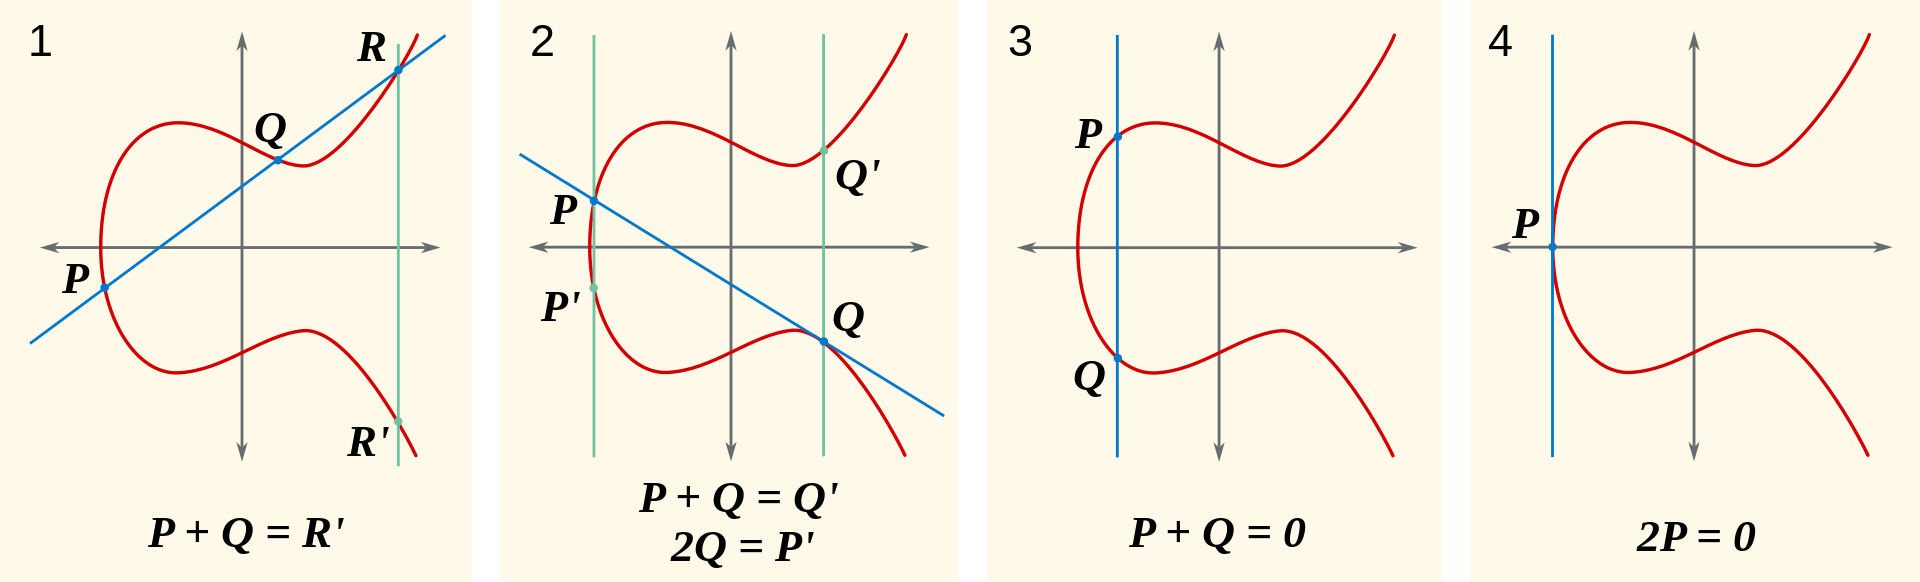
\includegraphics[width=\textwidth]{ecc_ops.png}
    \caption{Operace sčítání na eliptické křivce nad reálnými čísly pro různé případy. \\ Zdroj: \href{https://commons.wikimedia.org/wiki/File:ECClines-2.svg}{SuperManu},  \href{https://creativecommons.org/licenses/by-sa/3.0}{CC BY-SA 3.0}, via Wikimedia Commons}
    \label{fig:ecc_ops}
\end{figure}

Kryptografie navíc kromě definice křivky (vybrání vhodných parametrů $a,b$ z definice) volí \uv{výchozí bod} zvaný generátor, ležící někde na křivce. Křivky jsou definované nad zbytkovým tělesem a tak platí, že násobky generátoru tvoří tzv. cyklické podgrupy -- od určitého násobku (\uv{periody}) se body opakují. Více matematicky řečeno $\exists k \in \mathbb{N} \forall n \in \mathbb{N}: (n+k)G = nG$, kde $G$ je generátor. Takové nejmenší $k$ se nazývá řádem bodu $G$ a značí se $ord(G)$. Díky těmto vlastnostem je možné nalézt verzi problému diskrétního logaritmu pro eliptické křivky -- je snadné nalézt výsledek násobení $nG$, avšak zjistit násobitele $n$ z bodu $P=nG$ je obtížné. Proto jsou eliptické křivky vhodné pro asymetrickou kryptografii. Privátním klíčem v tomto schématu je právě skalár $n < ord(G)$ a veřejným klíčem bod $P=nG$. Kryptoanalytici hledají různé křivky a generátory s výhodnými vlastnostmi a ty následně pojmenovávají -- např. křivka, kterou se dále budeme zabývat, nese název \uv{secp256k1}.

\subsection{Reprezentace bodu na eliptické křivce}
Nejrelevantnější informací k této práci ohledně eliptických křivek je, že body lze reprezentovat různými souřadnicovými systémy. Přímočarý způsob je vyjádření souřadnic $x$ a $y$ jako bodu -- této reprezentaci se říká afinní. Existují ale například také projektivní nebo Jacobiho souřadnice. V projektivních souřadnicích je afinní bod $(X,Y)$ reprezentován jako $(ZX, ZY, Z)$ a v Jacobiho jako $(Z^2X, Z^2Y, Z)$. Důvodem těchto odlišných reprezentací je údajné zrychlení výpočtu násobení bodu skalárem: pro každou reprezentaci můžeme operace nad el. křivkami vyjádřit algebraicky. Afinní reprezentace ve výpočtech potřebuje hledat inverzní prvky $z^{-1} \text{mod}~ p$, kdežto projektivní i Jacobiho reprezentace si vystačí s násobením na zbytkové třídě. 

\section{Specifika práce}
Tato práce se zaměří na porovnání rychlostí různých výpočtů nad eliptickými křivkami dvou programových knihoven v jazyce Python3. První z knihoven, ECpy, implementuje různé křivky (nejen Weierstrassovské) a kryptografické metody nad nimi definované. Umí také načíst mnoho známých pojmenovaných křivek. Druhá knihovna, ECC.py, je autorská a implementuje pouze Weierstrassovské křivky, elektronické podepisování (ECDSA) a bezpečnou dohodu na symetrickém klíči (ECDH). Z pojmenovaných křivek zná akorát křivku secp256k1, používanou např. v bitcoinovém blockchainu. Knihovna ECpy používá při výpočtech nad Weierstrassovskými křivkami Jacobiho reprezentaci bodů, kdežto ECC.py standardní afinní. Výsledkem porovnání pak bude i ověření, zda je Jacobiho reprezentace skutečně výpočetně efektivnější.

Předmětem porovnávání budou samotné operace sčítání a dvoj-/násobení bodů, digitální podepisování a nalezení afinní souřadnice $y$ ze známého $x$, které obě knihovny rovněž podporují.

\section{Existující literatura}
O benchmarking eliptických křivek byly mnohé vyvedené snahy, většina z nich se však zaobírá odlišnými problémy. Nejčastější benchmarking probíhá okolo metod tzv. \uv{Zero-Knowledge Proof} nad eliptickými křivkami, jako např. párování (bilineárních zobrazení) dvou křivek \cite{bench-pair-ecc, snark-bench}, což se této práce vůbec netýká. Další studie porovnávají eliptické křivky se starším asymetrickým systémem RSA \cite{ecc-rsa-para-bench}. Jiné poměřují generování klíčů a bodů různých knihoven: \cite{vut-bench} měří časy generování bodů a násobení v různých knihovnách nad různými typy křivek na zařízeních Raspberry Pi Zero, 1, 2 a 3. Článek však spíše poskytuje kvantitu naměřených hodnot oproti kvalitě zpracování. Autoři článku \cite{ecdh-embedded-bench} měřili dobu generování klíčů a dohody na sdíleném klíči na zařízení STM32L476RG s knihovnou wolfSSL a své hodnoty porovnali s již naměřenými hodnotami knihovny CycloneCrypto. Práce \cite{mod-arti-bench} se také zabývá urychlením výpočtů nad eliptickými křivkami, ale o úroveň níže: snaží se vymyslet efektivní algoritmus na násobení čísel ve zbytkových třídách. Svůj navržený algoritmus následně porovnávají s algoritmem od SUN Microsystems.

Nejblíže této práci je článek \cite{eff-jacobi}, jehož autoři se snaží vyvinout algoritmy pro rychlejší násobení skaláry do hodnoty 31 v Jacobiho souřadnicích, navrhují nový souřadnicový systém EiSi a další algoritmy urychlující násobení včetně paralelizace. Své návrhy pak testují a porovnávají s jinými technikami v řadě experimentů. V žádném typu experimentu se však nevyskytují afinní a Jacobiho souřadnice vedle sebe, jsou porovnávány s dílem autorů separátně. Tabulka \ref{Tab:ejs} ze studie vyjímá počty operací násobení ze dvou různých experimentů. Jacobiho souřadnice se zdají být řádově efektivnější i do počtu násobení, avšak není jisté, zda dává smysl čísla obou sloupců navzájem porovnávat, jelikož autoři nerozebírají konkrétní podobu experimentů a tak se může jednat o naprosto odlišné případy. Číslo v názvu křivky odpovídá velikosti prvočísla zbytkové třídy v bitech (a tedy také privátního klíče).

\begin{table}[]
\centering
\begin{tabular}{|l|l|l|}
\hline
\textbf{Křivka} & \textbf{Afinní} & \textbf{Jacobi} \\ \hline \hline
P-521           & 478 056         & 13 312          \\ \hline
P-384           & 259 177         & 9 752           \\ \hline
P-256           & 115 340         & 6 488           \\ \hline
P-224           & 88 921          & 5 697           \\ \hline
\end{tabular}
\caption{Počet operací násobení pro afinní a Jacobiho souřadnice. Data pochází z dvou různých experimentů v \cite{eff-jacobi} -- jedná se o sjednocení zredukovaných tabulek 3 a 4. }
\label{Tab:ejs}
\end{table}

Žádná studie porovnávající přímo afinní a Jacobiho souřadnice nebyla nalezena, ani studie zaobírající se knihovnou ECpy.

\section{Návrh experimentů}
Experimenty budou implementovány v jazyce Python3, jelikož také obě benchmarkované knihovny jsou psány v tomto jazyce. Pro snadnou rozšiřitelnost vytvoříme dva skripty: první bude obsahovat benchmarky jako samostatné funkce a druhý skript pomocí inspekce spustí všechny testy prvního skriptu. Přidávání nových benchmarků tudíž znamená pouze jeho implementaci v prvním skriptu a žádné další akce.

Jak bylo nastíněno, každý benchmark je samostatná funkce jazyka Python3. Každá z funkcí bude mít nepovinný argument specifikující počet opakování daného testu s rozumnou výchozí hodnotou (1000). Každý benchmark bude testovat jednu funkcionalitu jedné knihovny -- každý benchmark tudíž bude \uv{duplikován} pro každou z knihoven zvlášť. Struktura každého experimentu pak bude následující:

\begin{lstlisting}[language=Python, caption=Struktura Experimentu]
    from time import perf_counter_ns
    
    def knihovna_benchmark(reps=1000, *dalsi_argumenty):
        # inicializace promennych spolecnych pro
        # kazdy z experimentu
        vars = init_vars()
        T = 0 # kumulativni doba vsech experimentu
        for _ in range(reps):
            # inicializace promennych konkretniho experimentu
            exp_vars = init_exp_vars(vars)
            t = perf_counter_ns()
            benchmark(exp_vars, vars)
            T += perf_counter_ns() - t
        # vraceni vysledku ve spravnem formatu
        return f"{knihovna},{benchmark},{T/reps}\n"
\end{lstlisting}

Při návrhu benchmarků zjišťujících rychlost nebo dobu trvání je důležité věnovat pozornost měření času. V počítačích existuje mnoho typů hodin, časovačů a oscilátorů, z nichž každý má jinou frekvenci nebo se aktualizuje v jiný moment. Nativní knihovny jazyka Python3 poskytují různé typy časovačů, z nichž nejvhodnější našemu účelu je \verb|time.perf_counter_ns()| -- inkrementuje se monotónně (neovlivňují ho systémové korekce) pouze za běhu procesu (ne když je procesor přidělen jinému procesu) a má vysoké rozlišení (dle dokumentace). Tento časovač se tak zdá být pro benchmarkování nejvhodnější. Všechny experimenty budou provedeny nad křivkou secp256k1. 

Výsledky benchmarků budou serializovány do řetězce, který funkce vrací. Řetězce budou po dokončení všech benchmarků zpracovány tak, aby výstupem programu byl dokument ve formátu CSV s hlavičkou \verb|benchmark;ecpy;ecc| -- v prvním sloupci název benchmarku, ve druhém průměrná doba trvání benchmarku pro knihovnu ECpy a ve třetím pro knihovnu ECC.py. Číselné hodnoty budou pro přehlednost po tisících odděleny čárkou, oddělovačem CSV souboru bude proto středník\footnote{formát je tedy spíše \uv{SSV} -- Semicolon-Separated Values}. Kromě formátu CSV bude benchmarkovací program také umět vygenerovat \LaTeX ~ tabulku podle argumentů na příkazové řádce.

\subsection{ECDSA}
Zkratka ECDSA znamená digitální podepisování pomocí eliptických křivek. Tento protokol implementují obě knihovny a tak se nabízí otestovat doby podepisování a ověření podpisu. Standardní algoritmus podpisu obsahuje jedno násobení bodu skalárem a další modulární operace včetně nalezení inverzního prvku. Tento algoritmus je však pravděpodobnostní, jelikož vyžaduje generování vhodného náhodného čísla. Při vygenerování nevhodného, což se zjistí až během výpočtu podpisu, je třeba algoritmus opakovat. V benchmarcích tak bude panovat jistá náhodnost doby běhu. Ověření podpisu je zcela deterministické bez náhody a utilizuje opět modulární operace vč. inverze a také dvě násobení bodu skalárem a sčítání bodů.

Experimenty nad každou knihovnou provedeme tří typů. Každý z nich benchmarkuje dobu jak podpisu, tak ověření. Kromě argumentu na počet opakování bude mít také argument na délku podepisované zprávy (výchozí hodnota 32 bytů) První typ experimentů bude zkoumat průměrnou dobu ECDSA pro stejnou podepisovanou zprávu (její hash) přes všechny opakování. Hash se nejprve náhodně vygeneruje (jako typ integer) a ve smyčce se mění akorát klíče, jimiž je zpráva podepisována. Druhý typ experimentu mění ve smyčce jak zprávu, tak klíče, a poslední typ mění pouze zprávu.

Benchmarky produkují dvě hodnoty a tak výsledný řetězec bude mít dva řádky. První řádek připojí za název benchmarku suffix \verb|sign| a druhý \verb|verify|, hodnoty budou odpovídající.

\subsection{Bodové operace}
Další várka experimentů ověřuje rychlost operací nad body křivky: sčítání, dvojnásobení a obecné násobení. Generování operandů implementujeme tak, že si necháme vygenerovat náhodné číslo menší než řád generátoru křivky a tímto číslem vynásobíme generátor. Zůstaneme tak pouze v cyklické grupě onoho generátoru, což platí i v praktické kryptografii eliptických křivek. Další možností by bylo vygenerovat náhodnou souřadnici $x$ a k ní najít odpovídající souřadnici $y$, čímž bychom mohli ověřovat i jiné body křivky. To ale není v praxi používáno a navíc ne každá $x$-ová souřadnice má odpovídající $y$-ovou -- generování bodu by tak mohlo zbytečně prodlužovat experimenty.

U benchmarků sčítání vygenerujeme dva body, které sečteme. Výsledek není nutné ukládat do žádné proměnné, jelikož interpreter jazyka Python3 musí sčítání vždy provést kvůli vedlejším efektům. Zaznamenaný čas tak přesněji odhadne dobu operace jako takové. U dvojnásobení bude stačit generovat jeden bod a pro obecné násobení vygenerujeme bod a skalár rovněž menší než řád generátoru.

\subsection{Zjištění $y$-ové souřadnice}
Obě knihovny podporují také nelezení $y$-ové souřadnice z $x$-ové. Souřadnici lze určit ze vztahu $y = \pm \sqrt{x^3 + ax + b}$. Výraz pod odmocninou snadno vypočteme ze zadané souřadnice a specifikace křivky, k odmocnině na zbytkové třídě modulo prvočíslem je třeba implementovat tzv. Tonelli-Shanksův algoritmus. Pro některá $x$ však dané $y$ nemusí existovat. Experimenty měří zejména dobu trvání implementace tohoto algoritmu. Experimenty tohoto typu budou dva. 

První experiment pouze generuje náhodná čísla ze zbytkové třídy křivky a měří čas algoritmu hledajícího odpovídající souřadnici, nezávisle na tom, zda pro vygenerované číslo existuje druhá souřadnice. Druhý experiment měří průměrný čas pouze z těch případů, kdy se vygenerovalo číslo $x$ s odpovídající souřadnicí $y$ -- neplatná čísla se přeskočí a pokusy se nezapočítávají do počtu opakování, běh tohoto benchmarku se tedy může náhodně prodlužovat.

\section{Výsledky a replikace}
V souladu s předešlou sekcí byly implementovány a spuštěny experimenty. Tato sekce rozebere jejich výsledky a rozebere manipulaci s benchmarkovací aplikací pro možnou replikaci experimentů.

\subsection{Výsledky}
Výstup benchmarkovací aplikace je zaznamenán v tabulce \ref{Tab:results-25000}. Hodnoty jsou průměrné doby trvání daného benchmarku v nanosekundách, časy byly průměrovány z 25 000 opakování každého benchmarku. Experimenty proběhly na zařízení s procesorem Intel Core i5-5300U pod 64bitovou verzí operačního systému Windows 10 Pro s dalšími běžícími procesy -- to je však díky použitému časovači irelevantní.

    \begin{table}[!ht]
        \centering
        \begin{tabular}{|c|c|c|}
            \hline
Benchmark & ECpy [ns] & ECC.py [ns] \\ \hline \hline
ECDSA podpis s konst. klíčem & 6,420,571.18 & 23,060,506.52 \\ 
ECDSA ověření s konst. klíčem & 12,904,788.91 & 46,025,457.98 \\ 
ECDSA podpis s konst. zprávou & 6,457,965.82 & 22,673,621.53 \\ 
ECDSA ověření s konst. zprávou & 12,939,980.20 & 45,040,922.67 \\ 
ECDSA podpis s var. zprávou & 6,390,056.55 & 22,997,217.87 \\ 
ECDSA ověření s var. zprávou & 12,820,902.94 & 45,690,935.96 \\ \hline
Nalezení $y$-ové souř. & 389,843.32 & 386,594.24 \\ 
Nalezení existující $y$-ové souř. & 471,788.96 & 532,413.66 \\ \hline
Sčítání bodů & 267,983.28 & 47,641.32 \\ 
Dvojnásobení bodů & 287,278.40 & 148,769.96 \\ 
Obecné násobení bodů & 6,186,594.40 & 23,093,736.81 \\ \hline
        \end{tabular}
        \caption{Výstup benchmarkovací aplikace s 25000 opakováními každého benchmarku}
        \label{Tab:results-25000}
    \end{table}

Nejdříve se zaměřme na bodové operace, jelikož se od nich odvíjí veškeré ECDSA benchmarky. Tabulka ukazuje, že sčítání bodů je v autorské knihovně ECC.py řádově rychlejší a operace dvojnásobení téměř dvakrát rychlejší i v afinních souřadnicích. Obecné násobení je ale téměř čtyřikrát pomalejší v knihovně ECC.py oproti ECpy. Tato skutečnost se na první pohled zdá paradoxní, jelikož obecné násobení závisí na předešlých dvou operacích. Obě knihovny navíc implementují stejný algoritmus násobení, zvaný \uv{Montogomeryho žebřík} (angl. Montgomery Ladder), pouze v jiných souřadnicových systémech. Navržené benchmarky pro sčítání a dvojnásobení důvod přímo neposkytují, avšak můžeme se jej pokusit odhadnout. Knihovna ECC.py při obou operacích počítá přímo nad afinními souřadnicemi, kdežto každá tato operace v knihovně ECpy musí afinní reprezentaci nejprve převést do Jacobiho souřadnic, v nich provést operaci a nakonec výsledek převést zpět do souřadnic afinních. Při obecném násobení však stačí udělat převod do Jacobiho souřadnic pouze před zahájením násobení a převod zpět provést až nad finálním výsledkem -- mezilehlé sčítání a dvojnásobení je prováděno přímo v Jacobiho souřadnicích. Soudě na základě této znalosti můžeme odhadnout, že knihovna ECpy je v izolovaném dvojení a sčítání pomalejší kvůli nutnosti převodu mezi souřadnicovými systémy. Toto naznačuje, že samotné operace v Jacobiho souřadnicích jsou rychlejší, ale převod výpočet znatelně zpomaluje. Ve světě kryptografie eliptických křivek se však téměř výlučně používá obecné násobení a tudíž jsou Jacobiho souřadnice prakticky výhodnější, což experimenty potvrzují. Ještě větší míru jistoty zajišťují experimenty nad algoritmem ECDSA, při nichž byla knihovna využívající Jacobiho souřadnice průměrně rychlejší (několikanásobně).

Zbylé benchmarky neověřují výhodnost Jacobiho souřadnic nad afinními, nicméně obě knihovny implementují testovanou metodu a tak byla do experimentů zahrnuta jako bonus. Jedná se o nalezení $y$-ové souřadnice ze znalosti $x$-ové tak, aby byla splněna rovnost z definice eliptické křivky. Obě knihovny implementují stejný algoritmus -- získají hodnotu pravé strany rovnice a pomocí Tonelli-Shanksova najdou její druhou odmocninu na modulární třídě. Obě implementace jsou si velmi podobné, avšak implementace ECC.py se snaží odstranit mnohá volání funkce mocnění, \verb|pow|, náhradou za rychlejší operace. Tonelli-Shanksův algoritmus často potřebuje zjistit obecnou mocninu dvou, která se dá realizovat bitovým posunem: $2^k = 1~<<~k$. Knihovna využívá této skutečnosti. Další rozdíl je v hlavní smyčce Tonelli-Shanksova algoritmu -- knihovna ECpy prochází řadu čísel cyklem \verb|for|, kdežto ECC.py používá \verb|while| cyklus. Výsledky benchmarků algoritmu (za předpokladu existujícího $y$) dávají najevo, že v jazyce Python3 je funkce \verb|pow| dobře optimalizovaná pro mocniny dvou, nebo je mnohem rychlejší cyklus \verb|for| anebo do nějaké míry platí oboje, neboť snaha o optimalizace v podobě bitových posuvů nebyla zdárná -- knihovna ECC.py byla ve hledání $y$ průměrně o něco pomalejší. 

\section{Instalace a spuštění experimentů}
Experimenty jsou implementovány v programovacím jazyce Python3 -- ten je potřeba mít nainstalovaný na zařízení. Kód je dostupný z \href{https://github.com/JustScrub/ecc_cli}{verzovacího systému git ve službě GitHub} \footnote{\url{https://github.com/JustScrub/ecc_cli}}. Experimenty jsou součástí většího projektu ECC CLI -- rozhraní z příkazové řádky okolo knihovny ECC.py a dalších nástrojů. Kód je možné stáhnout standardním způsobem pomocí nástroje git:

\begin{lstlisting}[language=bash]
    git clone https://github.com/JustScrub/ecc_cli.git 
\end{lstlisting}

V adresáři projektu je následně potřeba stáhnout závislosti pomocí balíčkovacího nástroje pip. Před tímto krokem je možné vytvořit virtuální prostředí \uv{venv} nebo \uv{conda}, aby se potřebné balíčky nestahovaly do globálního prostředí. Instalace závislostí je přímočará, nezapomeňme příkaz zavolat z adresáře nakolnovaného projektu:

\begin{lstlisting}[language=bash]
    pip install -r requirements.txt 
\end{lstlisting}

Nyní je instalace dokončena a můžeme spustit benchmarkování. Hlavní skript benchmarků se nachází v podadresáři benchmark, spustíme jej následujícím příkazem z kořenového adresáře projektu:

\begin{lstlisting}[language=bash]
    python3 benchmark/bench.py 25000
\end{lstlisting}

Příkaz spustí benchmarky, každý s 25 000 opakováními. Zadáním jiného čísla je možné počet opakování upravit. Bez dalších argumentů vytiskne skript výstup ve formátu CSV do terminálu po dokončení všech benchmarků. Programu je možné dodat další argumenty ve tvaru \verb|-c=csv_vystup.csv| nebo \verb|-l=latex_vystup.tex|. Za rovnítkem je cesta k souboru, do nějž se zapíše výstup v požadovaném formátu namísto do konzole. Příklad:

\begin{lstlisting}[language=bash]
    python3 benchmark/bench.py 25000 -c=vysledky.csv -l=vysledky.tex
\end{lstlisting}

\section{Závěr}
Cílem práce bylo ověřit pravdivost tvrzení, že výpočet operací nad body eliptických křivek je časově efektivnější v reprezentaci bodů pomocí tzv. Jacobiho souřadnic oproti klasické afinní reprezentaci. Různé zdroje zdůvodňují použití jiných reprezentací tímto tvrzením, avšak žádná z nalezených studií se nezhostila úkolu tvrzení empiricky podpořit. Tato práce proti sobě ověřila dvě knihovny implementující operace nad eliptickými křivkami reprezentující body v těchto systémech (afinní, resp. Jacobiho souřadnice). Z výsledků experimentů vzešlo ujištění, že Jacobiho reprezentace bodů je pro účely kryptografie eliptických křivek skutečně vhodnější, neboť i přes pomalejší transformace mezi souřadnicovými systémy se operace násobení bodů, která je v této kryptografii využívána ne-li exkluzivně, zdá být efektivnější v Jacobiho souřadnicích. Kromě této reprezentace existují také další, které se snaží předstihnout i operace v Jacobiho souřadnicovém systému.

\section{Bibliografie}
\printbibliography

\end{document}